\section{WAZIUP Platform}
Figure~\ref{fig-implem} presents a global overview of Waziup cloud platform stack, and its connection to IoT gateway through data broker (Orion Context Broker). The role of each component is presented, together with the technology selected in parenthesis.
The WAZIUP platform uses three distinct Cloud layers (in blue in the picture):
\begin{enumerate}
  \item “Infrastructure as a Service” (IaaS),    
  \item “Container as a Service” (CaaS),    
  \item and finally “Platform as a Service” (PaaS).     
\end{enumerate}

The first layer is provided by OpenStack. Its main role is to provide Virtual Machines (VMs), in which we run the full platform.
This layer is fundamental because most of Cloud vendors (Amazon, Rackspace) use VMs as basic selling units. The second layer is provided by Kubernetes. The role of this layer is to provide and serve containers, such as Docker containers, to WAZIUP services and applications. The containers provide light-weight and ultra-fast virtualization for applications and micro-services.
The containers themselves are running inside the VMs.
The third and final Cloud layer is provided by Deis. It provides services to developers, such as compiling and deploying of an application.
All the applications pushed by the users will be compiled with Deis and hosted in containers on Kubernetes.

\begin{figure}[htb]  
\centering  
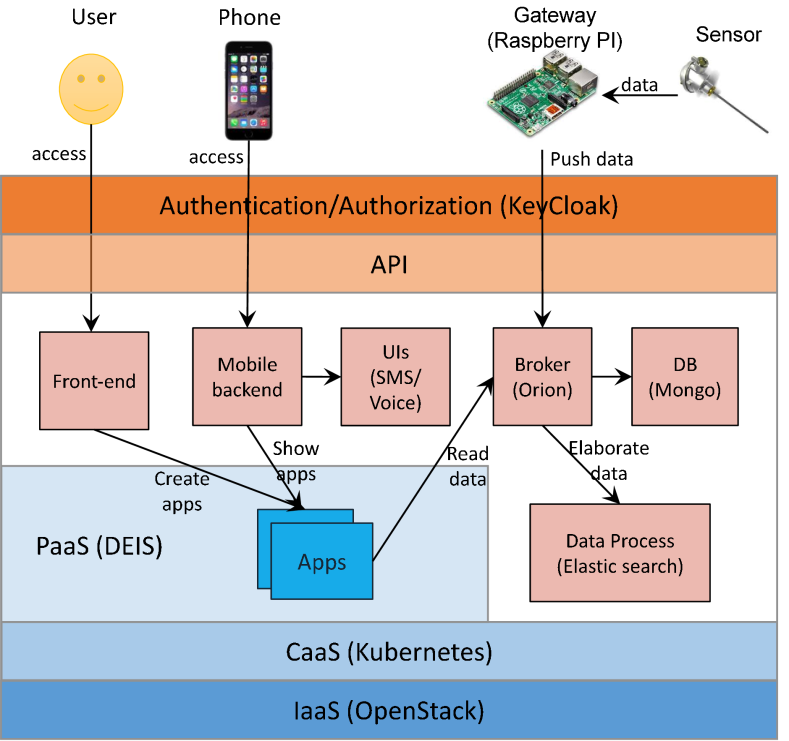
\includegraphics[width=.6\linewidth]{figures/CloudServicesArchitecture.png}   
\caption{Global overview of WAZIUP Cloud platform, and services}
\label{fig-implem}  
\end{figure}
The Gateway pushes sensors' data to the data broker, which is FIWARE Orion.
The data is distributed to the applications requesting it.
Orion also interfaces with the database and the data processing (Elastic Search), for historical data analysis.

Keycloak provides both Authentication and Authorization management.
For instance, when accessing the dashboard, the user need to provide a username and password.
This is provided by Keycloak authentication layer.
To access the platform, the users (Web, mobile) and external components (IoT gateway) need to go through the API server.
The API server exposes a common API for all the services of the Waziup platform.
Each of the endpoints of the API server is secured with Keycloak.

In addition, through the dashboard and APIs the user can access only sensors that are authorized for him.
This is enforced by Keycloak authorization layer.

Mobile phones are used to interfaces with the SMS and voice commands component.
This component allows Waziup applications to send SMS and voice notifications to the users.

In next sections, we present WAZIUP platform components in more details on security and data analytics.
\subsection{Platform Security Architecture}
IoT security has several dimensions; one is from communication between IoT devices and software platform; the other side is related to the whole software platform managing data, and services.

Figure \label{fig-services} illustrates WAZIUP services architecture in more details. The access to different WAZIUP services is performed by the WAZIUP APIs server (Dashboard API Server in Figure \label{fig-services}. The APIs server acts as a gateway placed in the demilitarized zone between the Internet and the internal network with WAZIUP services. WAZIUP APIs server provides public endpoints for the internally hosted services and proxies to them. All these services will not provide any Ingress to outside world. APIs Server can communicate with all Kubernetes internal services. And can respond to Client queries about different services. Thus, APIs Server will act as a proxy to provide security for WAZIUP services.


\begin{figure}[htb]
\centering
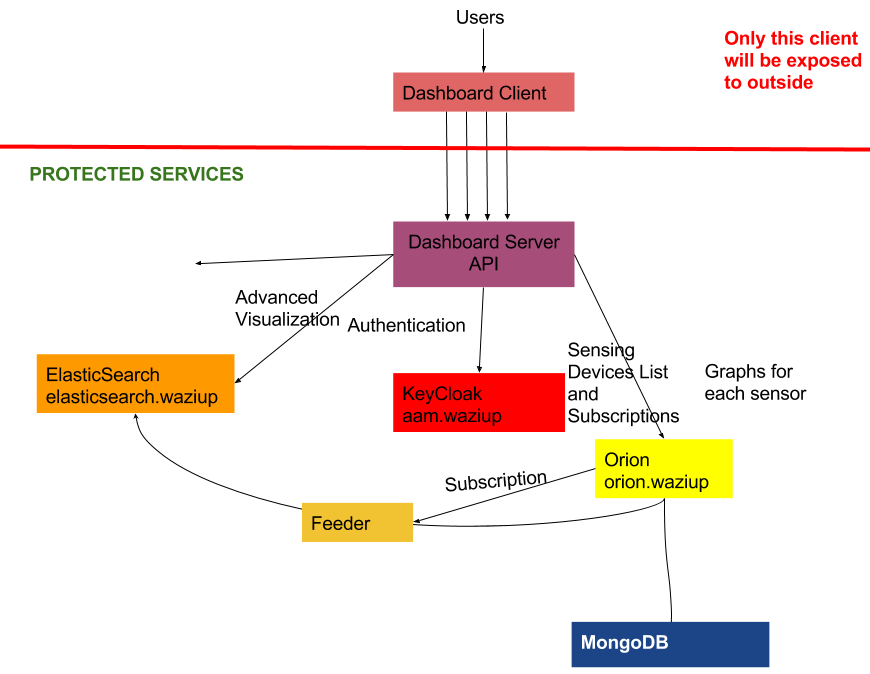
\includegraphics[width=.6\linewidth]{figures/ServicesArchitecture.png}
\caption{Detailed Picture of WAZIUP Cloud platform, and services architecture}
\label{fig-services}
\end{figure}

Authentication is the first requirement in implementing security. Users should be first identified by WAZIUP platform, then they can request access to different resources; that we call this step as authorization. WAZIUP APIs server takes care of the authentication and authorization of incoming requests from Internet. The authentication is performed with the help of Keycloak server. The authorization is done by the WAZIUP APIs server directly.
Depending on whether a service is accessed in an interactive manner (from the web-browser) or in a programmatic manner (directly from another service), WAZIUP APIs server provides two basic flows:
\begin{itemize}
\item Authentication for interactive use (e.g. from a Dashboard web client):
A user accesses a page (e.g. through a Dashboard web client). The browser sends a request to the APIs server. The server finds out that client has not authenticated yet and redirects the client’s browser to a login screen provided by Keycloak

User enters his/her credentials.
Keycloak validates the credentials, sends a request to APIs server notifying it that the user is authenticated and redirects user’s web-browser back to the original page.

When the WAZIUP APIs serves the web page now, it creates a session for the user and includes the access token to the session. The response to the client then includes a cookie with the session id.

Any subsequent request by the user includes the session id, which enables the WAZIUP APIs server to lookup the access token and validate the access.

\item Authentication for programmatic use (e.g. from a sensor gateway):
A user generates (typically through some web-based client) an offline access refresh token. The token is given to a device (e.g. the sensor gateway) as a configuration parameter.
When the device wants to make a request, it contacts Keycloak and requests an access token to be generated based on the refresh token.
Keycloak server provides an access token. (As opposed to the refresh token, the access token has rather limited duration of validity - typically in order of minutes.)
The device makes a request to a service endpoint (on the WAZIUP APIs server). As part of the request, it includes the following header (where access\_token is to be replaced by the actual access token received from Keycloak):
Authorization: bearer ACCESS\_TOKEN
\end{itemize}

Once the authentication is successful completed, the APIs server uses the access token to validate if the user/device has access to a particular resource.

For the sake of the authorization, every user has an attribute “permissions” (this is maintained by Keycloak). The attribute permissions attaches the the role of the user (admin, advisor or farmer) to resources (sensors, etc.) under a particular service path in Orion. 

Examples of values of the “permissions” attribute:
\begin{itemize}

\item "admin": admin access to anything regardless of the service path
\item "advisor: /FARM1; advisor: /FARM2" - advisor (i.e. read-write access) to anything under /FARM1 and /FARM2 service paths
\item "farmer: /FARM1" - farmer at /FARM1
\item The roles can be combined, such that a user gets different roles at different service paths: "advisor: /FARM1; advisor: /FARM2; farmer: /FARM2; farmer: /FARM3" 

\end{itemize}

Keycloak setup
The approach described above requires that every user has an attribute “permissions” in Keycloak. Moreover, Keycloak has to be set up to include the attribute “permissions” into tokens it provides (in particular the access token). This is because the WAZIUP APIs server inspects the access token and reads the “permissions” attribute from it. Then, it interprets the permissions attribute to authorize a user w.r.t. to a particular resource.

The particular steps to obey in Keycloak setup are the following:
\begin{verbatim}
Required setup for a “Client” in Keycloak:
Configure Mappers. Add there a mapper as follows:
Name: permissions
Mapper Type: User Attribute
User Attribute: permissions
Token claim name: permissions
Claim JSON Type: String
Add to ID token: ON
Add to access token: ON
Add to userinfo: ON
Download config under Clients/dashboard/Installation
Select "Keycloak OIDC JSON"
Copy the text to "keycloak.json" in the WAZIUP APIs project
Required setup a “User” in Keycloak:
Create a user as usual
Create a new attribute "permissions" in Attributes and fill it with the permissions specification as described above.
\end{verbatim}

\subsection{Data Management and Analytics Architecture}
WAZIUP architecture integrates Orion for providing current sensor values and Elasticsearch to keep the history (timeseries) of sensor values. The Elasticsearch Feeder service is responsible for transferring data (current sensor values) from Orion to Elasticsearch (for historical record keeping). Figure \label{fig-services} presents the place of Feeder between Orion and Elasticsearch.

Elasticsearch Feeder is written in NodeJS. It accesses Orion and Elasticsearch through their REST APIs. It allows transferring data from Orion to Elasticsearch either in periodic manner (e.g. every 5 minutes) or by subscription when data are recorded in Elasticsearch only if they change in Orion.

The Elasticsearch Feeder is configured by specifying a set of tasks, where each task defines the Orion’s service path along with sensors their attributes and maps it to an Elasticsearch’s index.  A commented example of the configuration is below. The configuration is provided in YAML:

\begin{verbatim}
# Defines the HTTP endpoint for subscriptions
# Has to be present, even if no subscription-triggerred tasks are defined below.
endpoint:
  # Unique ID of the Feeder instance
  id: feeder1
  # URL at which Feeder endpoint can be reached
  url: http://feeder
  # Host/port to which Feeder should bind
  host: 0.0.0.0
  port: 8000

# Defines the default ElasticSearch connection settings.
# Can be specialized in the same section in a task
elasticsearch:
  host: elasticsearch
  port: 9200

# Defines the default Orion connection settings. Can be specialized in the same section 
# in a task
orion:
  # MUST NOT end with slash
  uri: http://broker

# Defines (multiple) tasks. Each task defines sensors and target index 
# in ElasticSearch
tasks:
- trigger: subscription

#  Trigger types are: "time", "subscription"
#  If it is "time", Feeder periodically polls Orion with the period specified below
#  If it is "subscription", Feeder listens to notifications and recreates the
#    subscription every period below.
#  Renewal of the subscription includes new listing of sensors, which means that
#    after the "period" time
#  new sensors will be automatically included in the subscription.
#  Note that Orion sends a notification every time a subscription is recreated.

#  period: 5000

# Specifies the throttling (in seconds) when subscription is used. If not specified, no throttling will be applied.
# throttling: 5

#  Specifies task-level Orion settings
#  Entries from the global "orion" are used here as defaults. They can be overridden
#  here. The same way, the fields here can be moved to the global "orion".

  orion:
    service: waziup
    servicePath: /FARM1/TESTS

#  Specifies task-level Elasticsearch settings
#  Entries from the global "elasticsearch" are used here as defaults. They can be
#  overridden here. The same way, the fields here can be moved to global 
#  "elasticsearch".

  elasticsearch:
    index: test

#  Specifies the filter over the sensors discovered.
  filter:

#  If set, only entities listed below will be considered. If missing, no filtering by 
#  IDs is done
    ids:
    - WS_FARM1_Sensor2
    - WS_FARM1_Sensor3
    - WS_FARM1_Sensor4

#  If set, only attributes listed below will be considered. If missing, no filtering by 
#  attributes is done.
    attributes:
    - SM1
    - SM2

\end{verbatim}

\subsection{Applications Platform Architecture}
WAZIUP vision is to make it easy for IoT developers to develop new applications, dashboards and services. With WAZIUP APIs Server model, we will develop some generic proxy APIs services such as for Security (KeyCloak proxy API), Data Management (Orion proxy API), Data Analytics (ElasticSearch proxy API), etc. These APIs may be developed as part of WAZIUP APIs Server, or separate Service APIs. These are just proxy APIs calling the respective service APIs. Figure \ref{fig-app} presents this concept for realization of application templates.

We will move toward this architecture design at the Dashboard level. With that we can realize Application Development templates for IoT developers much simpler. We give them Development APIs and templates in order to develop their own customized Application. These APIs will be developed as a NodeJS server.

With that, instead of contacting Orion in Dashboard Client, it will call Orion API of WAZIUP Server API with some parameters, and will get for example the list of sensors, sensors data, subscriptions, etc.

This approach will make it easier for developers to develop new dashboards having in place these already well developed and tested APIs on top of Waziup Services.


\begin{figure}[htb]  
\centering  
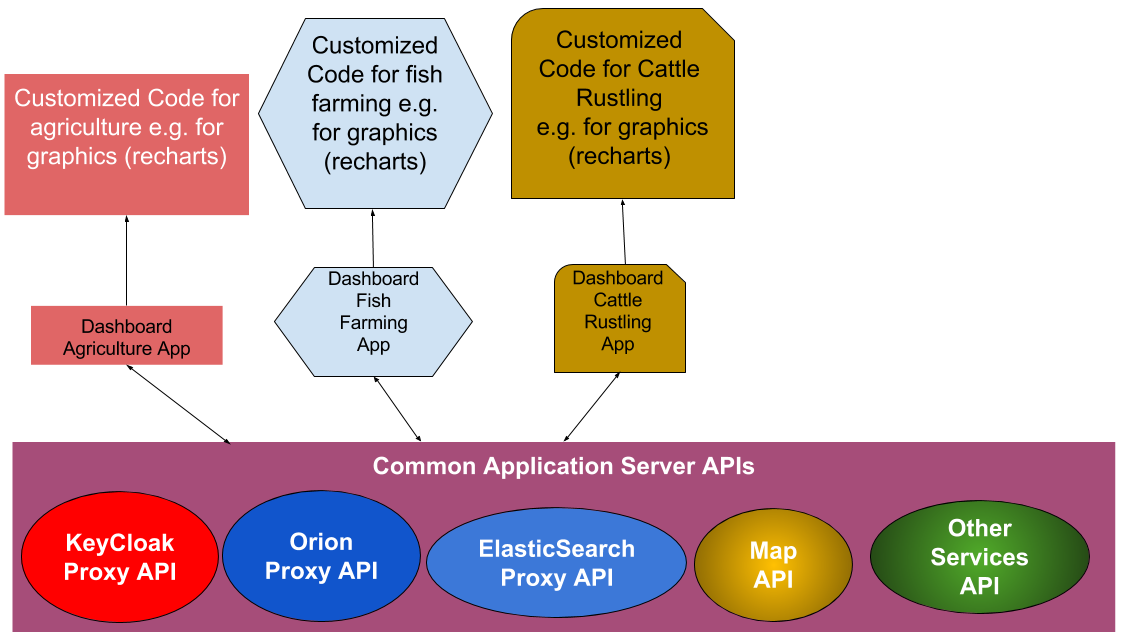
\includegraphics[width=.6\linewidth]{figures/AppArchitecture.png}   
\caption{A global view of WAZIUP Application Template platform}
\label{fig-app}
\end{figure}